\chapter{Related work}
\label{ch:related-work}

\section{Traditional and Learning-Based Program Repair}

Automated Program Repair (APR) has historically been dominated by search-based and constraint-based techniques. These methods treat repair as an optimization or constraint satisfaction problem, relying on test suites to validate candidate patches. They perform well on specific bug classes such as buffer overflows or integer errors, but fail on semantic errors that require understanding developer intent \citep{zhang2023surveylearningbasedautomatedprogram}.

The adoption of Large Language Models (LLMs) changed the approach fundamentally. Learning-based systems train on large code corpora and treat repair as a generation task, moving away from predefined templates and heuristic search \citep{yang2025surveyllmbasedautomatedprogram}.

\section{Prompting and LLM-Based Debugging}

Modern Automated Program Repair (APR) relies on Large Language Models (LLMs) built on the Transformer architecture \citep{vaswani2017attention}. The self-attention mechanism allows the model to weigh the importance of different tokens relative to one another regardless of their distance, which enables it to capture long-range dependencies between variable definitions and their usages and to model the syntax and semantics of programming languages \citep{austin2021program}.

Naive prompting fails on complex logical bugs. Researchers have developed conversational repair loops to address this. \citet{chen2023teaching} introduced \textit{Self-Debugging}, where an LLM is prompted to explain its code, identify errors based on execution feedback, and iteratively refine its own output. The approach is limited by the model's inability to observe actual runtime state.

Other frameworks go further by simulating human debugging workflows. \citet{zhong2024debug} proposed a "Debug like a Human" approach that forces the model to verify runtime execution step-by-step. By prompting the model to reason about control flow and variable states before generating a patch, these methods aim to reduce fixes that look syntactically correct but fail functionally.

Standard prompting approaches share a structural weakness: effective debugging requires both \textit{forward inference} (predicting outputs from inputs) and \textit{backward reasoning}, meaning deducing the root cause from an observed error state. Without execution traces, LLMs must perform this backward inference from static code alone, which is unreliable.

\section{Fine-Tuning on Runtime Information}

Researchers have also explored fine-tuning LLMs on datasets augmented with runtime information. The hypothesis is that exposing models to execution traces during training allows them to internalize the relationship between code structure and runtime behavior.

Recent empirical studies cast doubt on this approach. \citet{wang2025codesemanticshelpcomprehensive} conducted a comprehensive study on execution trace-based information, finding that appending trace data to the training context does not consistently improve repair performance for general-purpose code LLMs. They argue that the noise and complexity of raw traces can overwhelm the model's attention mechanisms. \citet{han2025rethinkingcapabilityfinetunedlanguage} re-evaluated fine-tuned models for vulnerability repair and found that standard fine-tuning often leads to overfitting on specific bug patterns rather than building an understanding of program semantics.

These results do not permit a simple conclusion. Appending raw traces and fine-tuning does not reliably improve repair performance. Work on execution-centric training suggests that models can learn substantially more about program semantics when trained to predict execution-relevant signals such as intermediate states, rather than when traces are treated as unstructured extra text \citep{armengolestape2025execution}. We treat fine-tuning as an open empirical question and focus primarily on inference-time use of runtime context.

\section{Agents}
\label{sec:agent-repair}

\citet{jimenez2023swebench} introduced SWE-bench, an evaluation framework of 2,294 software engineering problems drawn from real GitHub issues and pull requests across 12 popular Python repositories. Given a codebase and an issue description, a model must produce a patch that passes the associated test suite. When first published, the best-performing model, Claude 2, solved 1.96\% of issues. SWE-bench Lite is a 300-instance subset that has become the standard comparison point.

The dominant early approach treats repair as an interactive task. \citet{yang2024sweagent} introduced SWE-agent, which gives a language model a custom Agent-Computer Interface (ACI) with file viewing, editing, code search, and test execution. The model interacts with the repository iteratively, issuing commands and observing their outputs before producing a patch. This paradigm is an instance of the ReAct framework \citep{yao2022react}, which alternates Thought, Action, and Observation steps until the agent submits a result (Algorithm~\ref{alg:react}). SWE-agent reached 12.5\% pass@1 on SWE-bench Lite with GPT-4. \citet{zhang2024autocoderover} proposed AutoCodeRover, which replaces raw file navigation with AST-level code search and spectrum-based fault localization, allowing the model to retrieve class definitions and method signatures directly rather than reading entire files. AutoCodeRover reached 19\% pass@1 on SWE-bench Lite.

\begin{algorithm}[ht]
\caption{ReAct agent loop, the basis of interactive SWE agents \citep{yao2022react}.}
\label{alg:react}
\begin{algorithmic}[1]
\Require task $T$, tool set $\mathcal{A}$, max turns $K$
\Ensure patch or failure
\State context $\gets$ [\textsc{SystemPrompt}, $T$]
\For{$t = 1, \ldots, K$}
    \State thought $\gets \text{LLM}(\text{context})$ \Comment{model reasons about next step}
    \State action $\gets \text{LLM}(\text{context, thought})$ \Comment{selects tool and arguments}
    \If{action $= \textsc{Finish}(\textit{patch})$}
        \Return \textit{patch}
    \EndIf
    \State obs $\gets \text{Execute}(\text{action})$ \Comment{tool returns observation}
    \State context $\gets$ context $+$ [thought, action, obs]
\EndFor
\Return failure
\end{algorithmic}
\end{algorithm}

\citet{xia2024agentless} proposed Agentless, which replaces the interactive loop with a fixed three-phase pipeline: hierarchical fault localization (file, then function, then line), patch generation by sampling multiple candidates, and patch selection by re-running tests. The model does not choose its next action; the pipeline is fixed by the system. Agentless reached 32\% pass@1 on SWE-bench Lite at a cost of \$0.70 per instance, outperforming contemporary interactive agents at lower cost. The result shows that structured localization before generation carries more of the benefit than iterative interaction. \citet{yang2025kimidev} extended this with Kimi-Dev, which uses Agentless-style training as a skill prior. The model first trains on the structured pipeline to internalize localization, code editing, and self-reflection patterns, then adapts to agent interaction via fine-tuning on 5,000 publicly available trajectories. Kimi-Dev reached 60.4\% on SWE-bench Verified using the workflow approach and 48.6\% pass@1 with agent adaptation.

As reported pass@1 numbers have grown rapidly, several papers have raised concerns about what these numbers measure. \citet{liang2025sweillusion} showed that state-of-the-art models can identify the buggy file path from the issue description alone, without repository access, at up to 76\% accuracy. On repositories outside SWE-bench the same models drop to 53\%, suggesting that part of the apparent localization ability reflects memorization rather than reasoning. \citet{martinez2025dissecting} analyzed 178 leaderboard submissions and found that many systems do not disclose whether their pass@1 comes from a single attempt or from reranking across multiple sampled patches, making comparisons unreliable without transparent evaluation protocols.

\section{Code World Models}

\todo{Mentioning CWMs is good for overall review of approaches to codegen, but right now IMO it makes this chapter look a bit unfocused. Do we want to remove it?} APR research has moved toward systems called "Code World Models" that simulate the program's execution environment, treating code generation as a state-transition prediction task rather than text completion.

\begin{figure}[ht]
    \centering
    % Use the exact filename here. Extension .pdf can be omitted.
    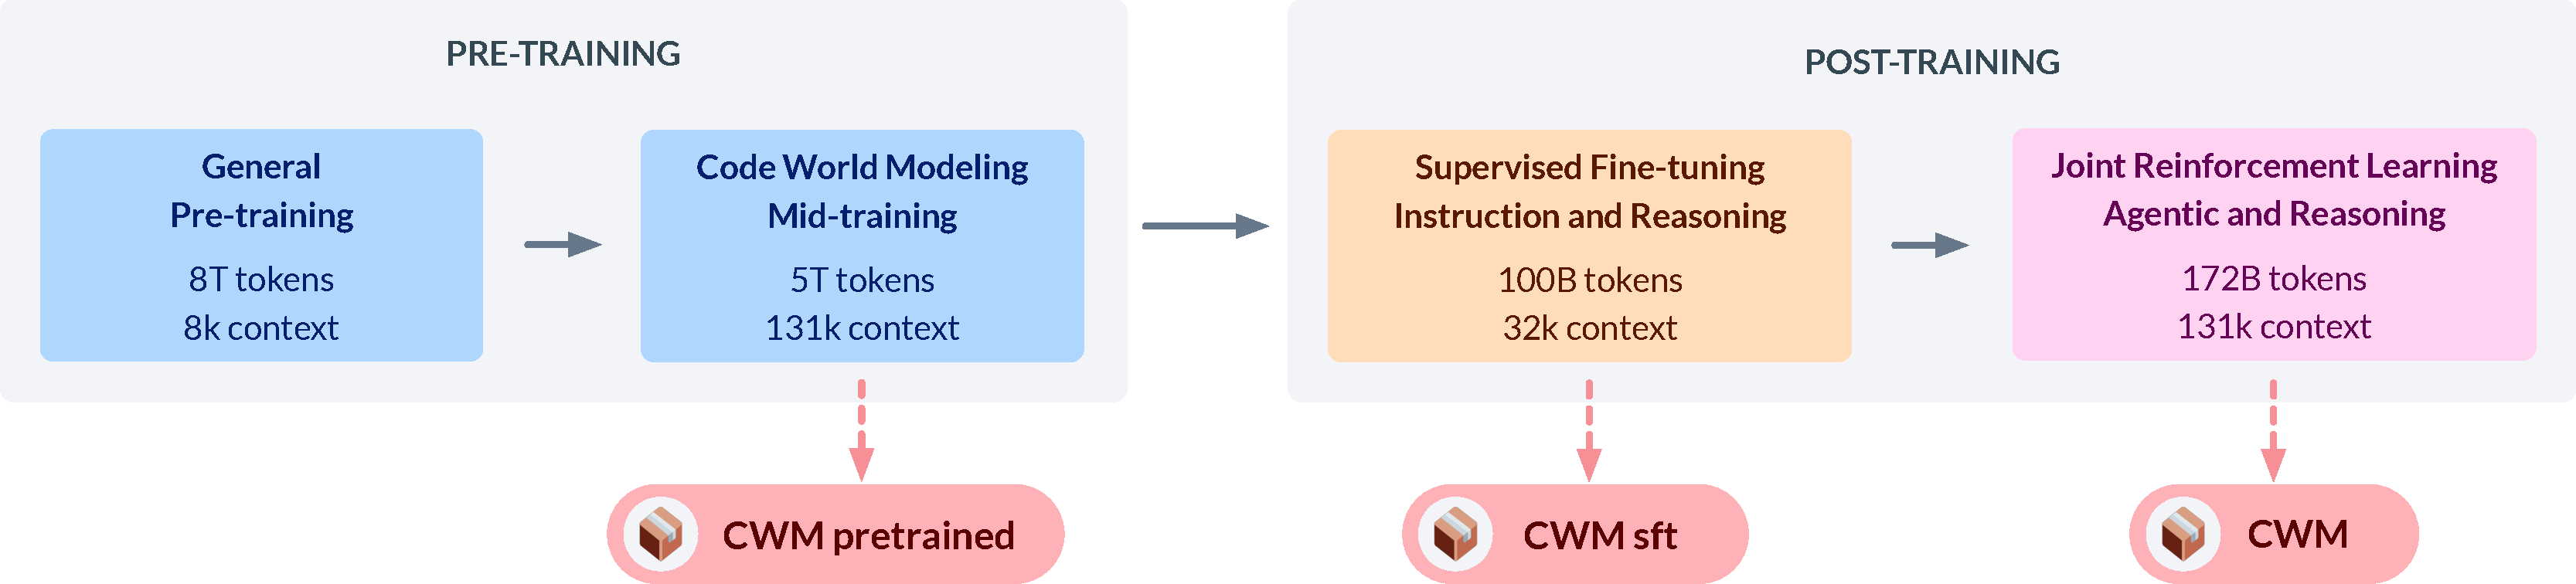
\includegraphics[width=1.0\textwidth]{figures/cwm_training_stages}
    \caption{The Code World Model (CWM) training pipeline. This diagram illustrates the three-stage process: general pre-training, mid-training on observation-action trajectories (including Python interpreter traces and agentic interactions), and final post-training/RL alignment \citep{cwm2025}.}
    \label{fig:cwm_stages}
\end{figure}

\subsection{Learning to Reason About Execution}
\citet{ni2024nextteachinglargelanguage} introduced \textit{NExT} (Naturalized Execution Tuning), a method that teaches LLMs to reason about code execution by generating natural language rationales derived from execution traces. By training the model to articulate the runtime behavior, NExT connects static code with dynamic logic.

\subsection{World Models as Simulators}
The most complete expression of this approach is the \textit{Code World Model (CWM)} \citep{cwm2025}. Unlike previous models that only see code text, CWM is trained on "observation-action trajectories" from interactive environments (such as Python interpreters and terminals). This allows the model to act as a simulator: given a current state and a code modification, it can predict the subsequent state of the system.

As illustrated in \cref{fig:cwm_stages}, moving from a general-purpose model to a world model requires exposure to the sequential trajectories of execution beyond instruction tuning. This exposure allows the model to map code edits directly to state changes.

This capability allows the agent to reason about the consequences of its edits across multi-file repositories and system-level interactions. These models are computationally expensive to train and deploy. This thesis explores a complementary direction: we investigate the effectiveness of injecting test-derived runtime contexts into the prompt at inference time, providing the runtime state to the model on demand rather than training it to simulate execution.
